\section{Introduction}
\label{sec:intro}

\begin{figure*}[t]
    \centering
    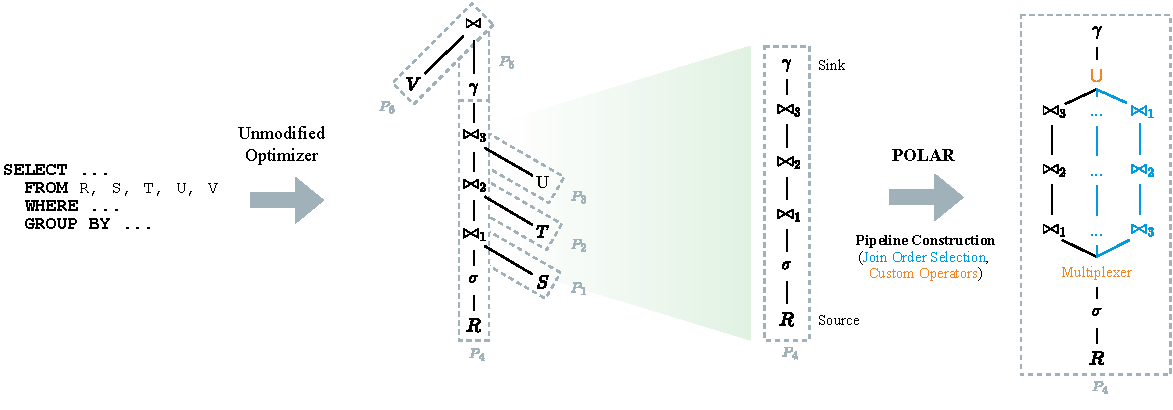
\includegraphics[width=0.82\textwidth]{figures/polar_pipeline-5.pdf}
		\vspace{-0.4cm}
		\caption{POLAR pipeline compilation from input query over standard, pipelined plan to POLAR pipeline.}
    \label{fig:pipeline_design}
		\vspace{-0.12cm}
\end{figure*}

% context
Cost-based query optimizations \cite{SelingerACLP79,moerkotte23} for selecting optimal join orders, join methods, and data access paths are crucial for the end-to-end performance of analytical queries. State-of-the-art exact join ordering algorithms such as DPsize~\cite{SelingerACLP79,HanKLLM08}, DPsub, DPcpp~\cite{MoerkotteN06}, and DPhyp~\cite{MoerkotteN08} rely on dynamic programming for efficient enumeration. These algorithms yield optimal execution plans, but only under the assumption of precise cardinality estimates.

\textbf{Cardinality Estimation Challenges:} Estimating precise cardinalities for intermediate results of complex queries remains a stubbornly difficult problem~\cite{LeisGMBK015}. First, most systems assume uniform distributions (no skew) and independence of predicates (no correlation) \cite{IlyasMHBA04}. These simplifying assumptions often cause under-estimation, which is problematic due to plan choices with poor asymptotic behavior~(\eg nested-loop joins), which perform poorly for larger intermediates \cite{IlyasMHBA04,LeisGMBK015}. Second, too coarse-grained statistics (\eg histograms \cite{KanneM10} or sketches \cite{IzenovDRS21}) may misrepresent clustered data. Third, user-defined functions and new environments (\eg federated, raw data) often do not allow obtaining statistics \cite{HueskePSRBKT12,JosifovskiSHL02,ReyFN23}. Fourth, complex queries with many operators are difficult to estimate because errors propagate exponentially \cite{IzenovDRS21,IoannidisC91,MoerkotteNS09}. Although recent work on ML-based estimators \cite{KipfKRLBK19,DuttWNKNC19,YangLKWDCAHKS19}, learning to distrust certain estimates \cite{MarcusNMZAKPT19}, and learning to rank plans \cite{BehrMK23} offer benefits, they do not solve all problems above.

\textbf{Adaptive Query Processing (AQP):} In the past two decades, a spectrum of AQP techniques \cite{BabuB05,DeshpandeIR07,IvesDR07,DeshpandeHR06} has been devised to address the challenges of unknown and changing data characteristics. Many AQP techniques follow the classical MAPE control loop of monitoring, analyzing, planning, and executing \cite{IvesDR07,mape05,AboulnagaHLLMPR04}. Existing techniques include inter-query optimization with learned cardinalities for expressions \cite{BrunoC02,ChenR94,StillgerLMK01}, late binding with re-optimization at pipeline breakers \cite{DeshpandeHR06} or parameter binding \cite{BizarroBD09}, inter-operator re-optimization at checkpoints \cite{KabraD98}, progressive and pro-active re-optimization with validity ranges \cite{MarklRSLP04,BabuBD05}, intra-operator adaptivity with union stitch-up plans \cite{IvesHW04}, intra-query adaptivity via reinforcement learning \cite{TrummerWMMJA19,TrummerWWMMJAR21,WeiT22}, as well as tuple routing policies in Eddies \cite{HellersteinA00,Arpaci-Dusseau03,Deshpande04,BizarroBDW05}. Many of these strategies require both optimizer and runtime extensions for effective and efficient adaptivity.

\textbf{Robust Query Processing:} An alternative mitigation strategy for poor cardinality estimates is robust query processing \cite{Haritsa20}. The influential Picasso project \cite{Haritsa10} on plan diagrams \cite{ReddyH05} revealed that state-of-the-art DBMS compile many very specialized plans that are only optimal in a small subspace of cardinalities. Since these cardinalities are difficult to estimate, robust query processing seeks to find a small number of plans that together cover a broad range of cardinalities \cite{DDH07,DDH08}. Despite a sequence of valuable improvements \cite{DDH08,AbhiramaBDSH10,GraefeGKP12,DuttH14} (including so-called plan bouquets \cite{DuttH14}), many of these strategies are offline approaches and largely intractable for intra-query or intra-operator adaptation during runtime \cite{Haritsa20}. 

\textbf{POLAR Overview:} Although AQP comprises many valuable ideas, only very few are implemented by data(base) systems in practice. We attribute this largely to the induced complexity of intertwining planning and execution, difficulties in testing and debugging, and potential performance regressions due to overheads of adaptivity. Inspired by tuple-routing and self-scheduling (queue-based) systems, we introduce POLAR as a novel adaptive processing approach of join pipelines. We enhance left-deep join pipelines with alternative join orders during planning, perform regret-bounded tuple routing for exploration, and process most data through \emph{plans of least resistance} (i.e., plans with few intermediates). In contrast to tuple routing in Eddies and SkinnerDB, POLAR is non-invasive to the optimizer and runtime, has low and bounded overhead, and does not require state management (e.g., partially-built hash tables).

\textbf{Contributions:} Our primary contribution is the concept of plans of least resistance (POLAR) as a new AQP technique designed for simple system integration and bounded overhead. Our detailed contributions include the novel POLAR design and its evaluation:
\begin{itemize}
    \item \emph{Pipeline Design:} We introduce a holistic, non-invasive pipe\-line design from objectives over pipeline compilation and join order selection to parallel pipeline processing with performance tracking (Section~\ref{pipeline-design}).
    \item \emph{Routing Strategies:} We propose an extensible multiplexer operator and several routing strategies, as well as describe their trade-offs and runtime characteristics (Section~\ref{sec:routing_strategies}).
		\item \emph{SSB-skew Benchmark:} As a basis for evaluating AQP systems on data with correlations and clustering, we introduce and share the new SSB-skew benchmark (\href{https://github.com/d-justen/duckdb-polr/tree/master/benchmark/ssb-skew}{SSB-skew repository}).
    \item \emph{Experiments:} Using a variety of benchmarks (JOB, SSB, SSB-skew), we systematically study the performance characteristics of a POLAR prototype in DuckDB~\cite{RaasveldtM19}. We evaluate different join order selection and routing strategies and compare with different AQP systems (Section~\ref{experiments}).
\end{itemize}
